\chapter{Data Access with  ADO (ActiveX Data Object) .\ NET}
ADO .\ NET provides consistent access to data sources such as SQL Server and XML, and to data sources exposed through OLEDB and ODBC. Data-sharing consumer applications can use ADO .\ NET to connect to these data sources and retrieve, handle, and update the data that they contain.

\section{Comparison Between ADO and ADO .\ NET}
\begin{longtable}[ht!]{@{}p{6cm}p{6cm}@{}}
\caption{Comparison between ADO and ADO .\ NET}\label{ado-vs-ado-dot-net} \\

\toprule
	\textbf{ADO} & \textbf{ADO .\ NET} \\
\midrule

\endfirsthead
\multicolumn{2}{c}%
{\tablename\ \thetable\ -- \textit{Continued from previous page}} \\
\hline
\textbf{ADO} & \textbf{ADO .\ NET} \\
\hline
\endhead \hline
\multicolumn{2}{r}{\textit{Continued on next page}} \\
\endfoot
\endlastfoot

ADO is based on Component Object
Modeling (COM) & ADO .\ Net is based on Common Language
Runtime (CLR) 
\tabularnewline

Stores data in binary format & Stores data in \verb|XML| format i.\ e.\  parsing of data 
\tabularnewline
Can't be integrated with \verb|XML| because ADO have limited access of \verb|XMLs| & Can be integrated with \verb|XML| as having robust support of \verb|XML| 
\tabularnewline
In ADO, data is provided by \texttt{RecordSet} & In ADO .\ Net data is provided
by \texttt{DataSet} or \texttt{DataAdapter}
\tabularnewline
ADO is connection oriented means it requires
continuous active connection & ADO .\ NET is disconnected, does not need continuous
connection
\tabularnewline
ADO gives rows as single table view, it scans
sequentially the rows using \texttt{MoveNext} method & ADO .\ NET gives rows as collections so you can access
any record and also can go through a table via loop
\tabularnewline
In ADO, You can create only Client side cursor & In ADO .\ NET, You can create both Client \& Server side cursor
\tabularnewline
%
Using a single connection instance, ADO cannot
handle multiple transactions & Using a single connection instance, ADO .\ NET can handle multiple transactions
\tabularnewline

\bottomrule

\end{longtable}


\emph{\textbf{Note}: A cursor is a temporary work area created in the system memory when a SQL statement is
executed. A cursor contains information on a select statement and the rows of data accessed by it.
This temporary work area is used to store the data retrieved from the database, and manipulate this
data. A cursor can hold more than one row, but can process only one row at a time. The set of rows the
cursor holds is called the \textbf{active set}.}




\section{ADO .\ NET Concept and Overview}
ADO .\ NET provides a bridge between the front end controls and the back end
database. The ADO .\ NET objects encapsulate all the data access operations and the controls interact with these objects to display data, thus hiding the details of
movement of data.

ADO .\ NET includes .\ NET Framework data providers for connecting to a database, executing commands, and retrieving results. Those results are either processed directly, placed in an ADO .\ NET \texttt{DataSet}. 


The ADO .\ NET classes are found in \texttt{System.Data.dll}, and are integrated with the \texttt{XML} classes found in \texttt{System.Xml.dll}.

\subsection*{Benefits of ADO .\ NET}

\begin{itemize}
	\item \textbf{Interoperability}
	
	Uses \texttt{XML} to transfer data across a network. This is not necessary that the destination	component should be a .\ NET application. Any receiving component that is able to read XML can read the
	data specified in the \texttt{XML} format.
	
	\item \textbf{Maintainability}
	
	Since ADO .\ NET is different layer and independent of database, it is loosely coupled with business logic, it enables easy transform of the architectural changes in a deployed application.
	
	\item \textbf{Performance}
	
	Provides fast execution of disconnected applications, over the disconnected \texttt{RecordSets} in classic ADO.
	
	\item \textbf{Scalability}
	
	Provides the conservation of resources, such as database locks and database connections.
	The applications that are based on ADO.NET support disconnected across to data. So, that the databases
	are not locked by user queries for long duration.
\end{itemize}
The Figure {\ref{fig:ado-dot-net-objects}} shows the ADO .\ NET objects at a glance:

\begin{figure}[ht]
	\centering
	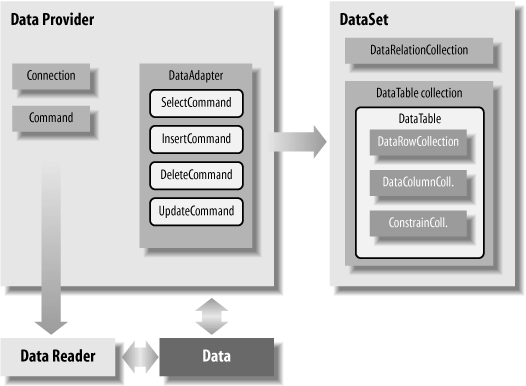
\includegraphics[width=0.9\textwidth]{ado-dot-net-architecture}
	\caption{ADO .\ NET Architecture.}\label{fig:ado-dot-net-objects}
\end{figure}

\subsection{ADO .\ NET Architecture}
The ADO.NET architecture has two main parts:
\begin{enumerate}
	\item \texttt{DataProvider} (Connected Objects or Connection oriented objects)
	\item \texttt{DataSet} (Disconnected objects or Connection-less objects)
\end{enumerate}


\subsubsection{DataProvider}
\begin{itemize}
	\item The .\ NET framework Data Provider is component that has been explicitly designed for data manipulation
	and fast, forward-only, read-only access to data.
	\item .\ NET Framework data provider is used for connecting to a database, executing commands, and retrieving
	results.
	\item The Data Provider has four core objects:
	\begin{enumerate}
		\item \textbf{Connection}: Establishes a connection to a specific data source
		\item \textbf{Command}: Executes a command against a data source
		\item \textbf{DataReader}: Reads a stream of data from a data source
		\item \textbf{DataAdapter}: Populates a data set and resolves updates with the data source
	\end{enumerate}
\end{itemize}
An ADO .\ NET data provider is a software component that interacts with a data source. ADO .\ NET
data providers are analogous to ODBC drivers, JDBC drivers, and OLE DB providers.

\noindent \emph{\textbf{Note}: ODBC (Open Database Connectivity) is designed to provide access primarily to SQL data in a multi-
platform environment. OLE DB (Object Linking and Embedding Database) is designed to provide access to all
types of data in an OLE Component Object Model (COM) environment. OLE DB includes the SQL functionality
defined in ODBC but also defines interfaces suitable for gaining access to data other than SQL data.}


\paragraph*{Connection}
\begin{itemize}
	\item The Connection object is the first component of ADO .\ NET.
	\item The Connection objects provider connectivity to a data source.
	\item It establishes a connection to a specific data source.
	\item Connection object helps in accessing and manipulating a database.
	\item The base class for all Connection objects in the \texttt{DbConnection} class.
	\item Example: See Section \ref{sec:connection}.
\end{itemize}

\paragraph*{Command}
\begin{itemize}
	\item The Command object enables access to database commands to return data, modify data, run stored procedures, and send or retrieve parameter information.
	\item It executes a command against a data source. Exposes Parameters and can execute in the scope of a Transaction from a Connection.
	\item You can execute SQL queries to return data in a \texttt{DataSet} or a \texttt{DataReader} object.
	\item Command object performs the standard Select, Insert, Delete and Update T-SQL operations.
	\item The base class for all Command objects is the \texttt{DbCommand} class.
	\item Example: See Section \ref{sec:command}.
\end{itemize}

\paragraph*{DataReader}
\begin{itemize}
	\item The Data Reader provides a high-performance stream of data from the data source.
	\item It reads a forward-only, read-only stream of data from a data source.
	\item \texttt{DataReader} object works in connected model.
	\item The base class for all \texttt{DataReader} objects is the \texttt{DbDataReader} class.
	\item Example: See Section \ref{sec:data-reader}.
\end{itemize}

\paragraph*{DataAdapter}
\begin{itemize}
	\item The Data Adapter provides the bridge between the Data Set object and the data source.
	\item The Data Adapter uses command object to execute SQL commands at the data source to both load the Data Set with data and reconcile changes that were made to the data in the dataset back
	to the data source.
	\item It populates a \texttt{DataSet} and resolves updates with the data source.
	\item The base class for all \texttt{DataAdapter} objects is the \texttt{DbDataAdapter} class.
\end{itemize}

\noindent The following lists the data providers that are included in the .\ NET framework.

\begin{enumerate}
	\item SQL Server
		\begin{itemize}
			\item Provides data access for Microsoft SQL server.
			\item Uses the \texttt{System.Data.SqlClient} namespace.
		\end{itemize}
	\item OLEDB
		\begin{itemize}
			\item For data sources exposed by using OLEDB.
			\item Uses the \texttt{System.Data.OleDb} namespace
		\end{itemize}
	\item ODBC
		\begin{itemize}
			\item For data sources exposed by using ODBC.
			\item Uses the \texttt{System.Data.Odbc} namespace.
		\end{itemize}
	\item Oracle
	\begin{itemize}
		\item For Oracle data sources.
		\item Uses the \texttt{System.Data.OracleClient} namespace.
	\end{itemize}
\end{enumerate}
Following Code demonstration of binding \texttt{GridView} control using Connection Oriented Objects of ADO .\ Net.

\lstinputlisting[caption=Example of GridView control using connection oriented objects]{ConnectionOrientedADO.cs}

\subsubsection{DataSet}
\begin{itemize}
	\item The dataset represents a subset of the database. 
	\item The dataset is a memory-resident representation of data that provides consistent relational programming
	\item It does not have a continuous connection to the database. 
	\item To update the database a re-connection is required. 
	\item The dataset represents a complete set of data, including related tables, constraints, and relationship
	among the table.
	\item The \texttt{DataSet} contains:
	\begin{enumerate}
		\item \texttt{DataTable} objects and 
		\item \texttt{DataRelation} objects. 
	\end{enumerate}

\end{itemize}

\paragraph*{DataRelation}
\begin{itemize}
	\item The \texttt{DataRelation} objects	represent the relationship between two tables.
	\item A relationship represented by the Data relation object, associated rows in one Data table with rows in another Data table.
	\item A relationship is analogous to a join path that might exist between primary and foreign key columns in a relational database.
	\item A data relation identifies matching columns in two tables of a dataset.
	\item The essential element of a data relation are:
		\begin{itemize}
			\item The name of the relationship
			\item The name of the tables being related
			\item The related column in each table
		\end{itemize}
	\item Relationship can be built with more than one column per table by specifying an array of Data Column objects as the key columns.
	\item Optionally, a Unique key constraint can be added to enforce integrity constraints when changes are made to related column values.
\end{itemize}


\noindent Listing \ref{lst:disconnected-objects-example} example demonstrate disconnected objects.

\lstinputlisting[label={lst:disconnected-objects-example}, caption=Example of disconnected objects]{DisconnectedADO.cs}


\paragraph*{DataTable}
\begin{itemize}
	\item The \texttt{DataTable} class represents the tables in the database. 
	\item A Data table is defined in the \texttt{System.Data} namespace and represents a single table of memory-resident data.
	\item It has the important properties as shown in Table \ref{tab:data-table-prop}; most of these properties are read only properties except the \texttt{PrimaryKey} property.
\end{itemize}


\begin{table}[ht!]
\centering	
	\caption{DataTable properites}\label{tab:data-table-prop}
\begin{tabular}{p{3cm}p{9cm}}
	\toprule
	\textbf{Properties}    & \textbf{Description}                                              \\ \midrule
	\verb|ChildRelations|  & Returns the collection of child relationship                      \\
	\verb|Columns|         & Returns the Columns collection                                    \\
	\verb|Constraints|     & Returns the Constraints collection                                \\
	\verb|DataSet|         & Returns the parent \texttt{DataSet}                                        \\
	\verb|DefaultView|     & Returns a view of the table                                       \\
	\verb|ParentRelations| & Returns the \texttt{ParentRelations} collection                            \\
	\verb|PrimaryKey|      & Gets or sets an array of columns as the primary key for the table \\
	\verb|Rows|            & Returns the Rows collection                                       \\ \bottomrule
\end{tabular}
\end{table}

\subparagraph*{DataRow}
The \texttt{DataRow} object represents a row in a table. It has the important properties as shown in Table \ref{tab:data-row-prop}:

\begin{table}[ht!]
	\centering
	\caption{DataRow properites}\label{tab:data-row-prop}
\begin{tabular}{p{3cm}p{9cm}}
	\toprule
	\textbf{Properties} & \textbf{Description}                                         \\ \midrule
	\texttt{HasErrors}  & Indicates if there are any errors relationship               \\
	\texttt{Items}      & Gets or sets the data stored in a specific column collection \\
	\texttt{ItemArrays} & Gets or sets all the values for the row                      \\
	\texttt{Table}      & Returns the parent table                                     \\ \bottomrule
\end{tabular}
\end{table}



%\subsubsection*{The DataAdapter Object}
%The DataAdapter object acts as a mediator between the DataSet object and the database. This helps the Dataset
%to contain data from multiple databases or other data source.
%
%\subsubsection*{The DataReader Object}
%The DataReader object is an alternative to the DataSet and DataAdapter combination. This object provides a
%connection oriented access to the data records in the database. These objects are suitable for read-only access,
%such as populating a list and then breaking the connection. \par 
%
%DataReader is read-only and forward only, meaning
%once you read a record and go to the next record, there is no way to go back to the previous record. It is also
%not possible to change the data using DataReader. DataReader is connection oriented, meaning it requires an
%active connection to the data source, while reading data. The forward-only nature of DataReader is what makes
%it an efficient choice to read data.

%\subsubsection*{DbCommand and DbConnection Objects}
%The \verb|DbConnection| object represents a connection to the data source. The connection could be shared among
%different command objects.
%\par
%
%The \verb|DbCommand| object represents the command or a stored procedure sent to the database for retrieving or
%manipulating data. \par

\section{Working with Connection, Command, DataReader}
An application needs to perform following steps to retrieve data from database:
\begin{enumerate}
\item  \textit{Connect to the Database}
\item  \textit{Prepare an SQL Command}
\item  \textit{Execute the Command}
\item  \textit{Retrieve the results and display in the application}
\end{enumerate}

\begin{itemize}
	\item The combination of \texttt{Connection}, \texttt{Command} and \texttt{DataReader} object gives us connected approach of
	connecting to database.
	\item Notice that we are using \texttt{SQLConnection}, \texttt{SQLCommand} and \texttt{SQLDataReader} classes. All the objects
	are prefixed with the word SQL. All these classes are present in \verb|System.Data.SqlClient| namespace. So,
	we can say that the .NET data provider for SQL Server is \verb|System.Data.SqlClient|.
	\item Sample ADO .\ NET code to connect to SQL Server Database and retrieve data using connection, command and \texttt{DataReader}:

	\lstinputlisting[caption={Example to connect sql server database and retrieve data using connection, command and reader}]{DbConnectionExample.cs}
	
	\item Sample ADO .\ NET code to connect to Oracle Database and retrieve data using connection, command and \texttt{DataReader}:
	
\begin{lstlisting}
	OracleConnection con = new OracleConnection("Oracle db Connection String");
	OracleCommand cmd = new OracleCommand("Select * from tblProduct", con);
	con.Open();
	OracleDataReader rdr = cmd.ExecuteReader();
	GridView1.DataSource = rdr;
	GridView1.DataBind();
	con.Close();
\end{lstlisting}
	Notice that we are using \texttt{OracleConnection}, \texttt{OracleCommand} and \texttt{OracleDataReader} classes. All the
objects are prefixed with the word Oracle. All these classes are present in \texttt{System.Data.OracleClient}
namespace. So, we can say that the .\ NET data provider for Oracle is \texttt{System.Data.OracleClient}.

\item Another example of using \texttt{DataReader} to load data:

\lstinputlisting[caption= {DataReader example}]{data-reader-example-2.cs}

If for some reason, you want to loop through each row in the \texttt{SqlDataReader} object, then use
the \texttt{Read()} method, which returns true as long as there are rows to read. If there are no more rows to
read, then this method will return false. In the following example, we loop through each row in
the \texttt{SqlDataReader} and then compute the 10\% discounted price.

\end{itemize}


\emph{If we want to connect to OLEDB datasources like Excel, Access etc, we can use OleDbConnection, OleDbCommand and OleDbDataReader classes. So, \. NET data provider for OLEDB is \texttt{System.Data.OleDb}.}

\subsubsection*{Different .NET Data Providers}
\begin{itemize}
	\item Data Provider for SQL Server - \texttt{System.Data.SqlClient}
	\item Data Provider for Oracle - \texttt{System.Data.OracleClient}
	\item Data Provider for OLEDB - \texttt{System.Data.OleDb}
	\item Data Provider for ODBC - \texttt{System.Data.Odbc}
\end{itemize}


Depending on the provider, the following ADO .\ NET objects have a different prefix:
\begin{multicols}{2}
		\begin{enumerate}
		\item \textit{Connection}: 
		\begin{itemize}
			\item \texttt{SQLConnection}, 
			\item \texttt{OracleConnection}, 
			\item \texttt{OleDbConnection}, 
			\item \texttt{OdbcConnection}, etc.
		\end{itemize}
	
		\item \textit{Command}: 
		\begin{itemize}
			\item \texttt{SQLCommand}, 
			\item \texttt{OracleCommand}, 
			\item \texttt{OleDbCommand}, 
			\item \texttt{OdbcCommand}, etc.
		\end{itemize}
	\item \textit{DataReader}: 
		\begin{itemize}
			\item \texttt{SQLDataReader}, 
			\item \texttt{OracleDataReader}, 
			\item \texttt{OleDbDataReader}, 
			\item \texttt{OdbcDataReader}, etc.
		\end{itemize}

		\item \textit{DataAdapter}: 
		\begin{itemize}
			\item \texttt{SQLDataAdapter}, 
			\item \texttt{OracleDataAdapter}, 
			\item \texttt{OleDbDataAdapter}, 
			\item \texttt{OdbcDataAdapter}, etc.
		\end{itemize}
	\end{enumerate}
\end{multicols}


\subsection{Connection}\label{sec:connection}
\begin{itemize}
	\item It is used to establish an open connection to the SQL Server database. 
	\item It is a sealed class. So, it cannot be inherited. 
	\item \texttt{SqlConnection} class uses \texttt{SqlDataAdapter} and \texttt{SqlCommand} classes together to increase performance when connecting to a Microsoft SQL Server database.
	\item Connection does not close explicitly even it goes out of scope. Therefore, you must explicitly close the connection by calling \texttt{Close()} method.	
	\item \texttt{Using} block is used to close the connection automatically. 
	\item We don't need to call \texttt{Close()} method explicitly, \texttt{Using} block do this for ours program implicitly when the code exits the block.
\end{itemize}

\subsubsection*{Example}
\begin{lstlisting}
using (SqlConnection con = new SqlConnection(connectionString)) {    
	con.Open();         
} 
\end{lstlisting}



\lstinputlisting[caption={Example of sqlConnection}]{sqlConnectionExample.cs}

\subsection{Command}\label{sec:command}
\begin{itemize}
	\item This class is used to store and execute SQL statement for SQL Server database. 
	\item It is a sealed class. So, it cannot be inherited.
\end{itemize}

\subsubsection*{Example}
\lstinputlisting[caption={Example of sqlCommand}]{sqlCommandExample.cs}



\subsection{DataReader}\label{sec:data-reader}
\begin{itemize}
	\item This class is used to read data from SQL Server database. 
	\item It reads data in forward-only stream of rows from a SQL Server database. 
	\item It is sealed class so that cannot be inherited. 
	\item It inherits \texttt{DbDataReader} class and implements \texttt{IDisposable} interface.
\end{itemize}



\lstinputlisting[caption={Example of sqlDataReaderExample.}]{sqlDataReaderExample.cs}


\section{Working With Dataset}
\begin{itemize}
	\item The ADO .\ NET \texttt{DataSet} is a memory-resident representation of data that provides a consistent relational
	programming model regardless of the source of the data it contains. 
	\item A \texttt{DataSet} represents a complete set of data including the tables that contain, order, and constrain the data, as well as the relationships
	between the tables.
	\item There are several ways of working with a DataSet, which can be applied independently or in combination.
	 We can:
	 \begin{itemize}
	 	\item Programmatically create a \texttt{DataTable}, \texttt{DataRelation}, and Constraint within a \texttt{DataSet} and populate the tables with data.
	 	\item Populate the \texttt{DataSet} with tables of data from an existing relational data source using a \texttt{DataAdapter}.
	 	\item Load and persist the \texttt{DataSet} contents using \texttt{XML}.
	 \end{itemize}
\end{itemize}


\subsection*{Creating DataSet Programatically}
\begin{itemize}
	\item In this program, we create two \texttt{DataTables}. 
	\item One stores two rows of patient information. 
	\item And the second stores two rows of medication information.
	\item We create a \texttt{DataSet} with the \texttt{DataSet} constructor. 
	\item Then we add the two \texttt{DataTables} to the \texttt{DataSet} instance. 
	\item Finally we print the \texttt{XML}.
\end{itemize}

\lstinputlisting[caption={Creating DataSet}, label={lst:dataset-example}]{dataset-example.cs}

\lstinputlisting[language=xml, caption={Output from Listing \ref{lst:dataset-example}}]{dataSetOutput.xml}


\subsection*{Populating DataSet with tables from database}
\begin{itemize}
	\item Following program send query to stored procedure in database and loads the table data into dataset. 
	\item The stored procedure for this would be:
\end{itemize}


\begin{lstlisting}[language=sql]
Create procedure spGetProductAndCategoriesData
as
	Begin
	Select ProductId, ProductName, UnitPrice
	from tblProductInventory
	Select CategoryId, CategoryName
	from tblProductCategories
End
\end{lstlisting}

And the program is illustrated in Listing \ref{lst:populate-dataset-database} calls stored procedure and loads data into dataset.

\begin{lstlisting}[caption={Loading data into DataSet using}, label={lst:populate-dataset-database}]
string ConnectionString = ConfigurationManager.ConnectionStrings["DBConnectionString"].ConnectionString;
using(SqlConnection connection = new SqlConnection(ConnectionString)) {
	SqlDataAdapter dataAdapter = new SqlDataAdapter("spGetProductAndCategoriesData", connection);
	dataAdapter.SelectCommand.CommandType = CommandType.StoredProcedure;
	DataSet dataset = new DataSet();
	dataAdapter.Fill(dataset);
	GridViewProducts.DataSource = dataset.Tables[0];
	GridViewProducts.DataBind();
	GridViewCategories.DataSource = dataset.Tables[1];
	GridViewCategories.DataBind();
}
\end{lstlisting}

\section{Adding, Deleting and Modifying Records in Dataset}
You edit data in data tables (\texttt{DataSet}) much like you edit the data in a table in any database. The process can include
inserting, updating, and deleting records in the table.

\subsection*{Editing/Modifying records:}
To edit an existing row in a \texttt{DataTable}, you need to locate the \texttt{DataRow} you want to edit, and then assign the updated
values to the desired columns. If you don't know the index of the row you want to edit, use the \texttt{FindBy} method to search
by the primary key.

\subsection*{Adding records:}
To add new records to a dataset, create a new data row by calling the method on the \texttt{DataTable}. Then add the row to
the \texttt{DataRow} collection (Rows) of the \texttt{DataTable}.

\subsection*{Deleting records:}
Call the Delete method of a DataRow.

\subsection*{Example}
\lstinputlisting[caption=CRUD operation in dataset]{dataset-crud.cs}


\section{Using DataView}
\begin{itemize}
	\item A \texttt{DataView} enables you to create different views of the data stored in a \texttt{DataTable}, a capability that is often used
	in data-binding applications. 
	\item Using a \texttt{DataView}, you can expose the data in a table with different sort orders, and	you can filter the data by row state or based on a filter expression.
	\item A \texttt{DataView} provides a dynamic view of data in the underlying \texttt{DataTable}: 
	\begin{itemize}
		\item the content, ordering, and membership reflect changes as they occur. 
	\end{itemize}
	\item This behavior differs from the Select method of the \texttt{DataTable}, which returns a \texttt{DataRow} array from a table based on a particular filter and/or sort order:
\begin{itemize}
	\item this content reflects changes to the underlying table, but its membership and ordering remain static. 
\end{itemize}
	\item The dynamic capabilities of the \texttt{DataView} make it ideal for data-binding applications.
	\item A \texttt{DataView} provides you with a dynamic view of a single set of data, much like a database view, to which you can apply different sorting and filtering criteria. Unlike a database view, however, a \texttt{DataView} cannot be treated as a table and cannot provide a view of joined tables. You also cannot exclude columns that exist in the source table, nor can you append columns, such as computational columns, that do not exist in the source table.
	
	\item You can use a \texttt{DataViewManager} to manage view settings for all the tables in a \texttt{DataSet}. 
	\item The \texttt{DataViewManager} provides you with a convenient way to manage default view settings for each table. When binding a control to more than one table of a \texttt{DataSet}, binding to a \texttt{DataViewManager} is the ideal choice.
\end{itemize}




\subsection*{Creating DataView}
There are two ways to create a \texttt{DataView}. You can use the \texttt{DataView} constructor, or you can create a reference
to the \texttt{DefaultView} property of the DataTable. The \texttt{DataView} constructor can be empty, or it can take either a
\texttt{DataTable} as a single argument, or a \texttt{DataTable} along with filter criteria, sort criteria, and a row state filter.

The following code example demonstrates how to create a \texttt{DataView} using the \texttt{DataView} constructor. A \texttt{RowFilter},
\texttt{Sort} column, and \texttt{DataViewRowState} are supplied along with the \texttt{DataTable}.


\begin{lstlisting}
DataView custDV = new DataView(custDS.Tables["Customers"], "Country = 'Nepal'", "ContactName", DataViewRowState.CurrentRows);
\end{lstlisting}

The following code example demonstrates how to obtain a reference to the default DataView of a DataTable using the DefaultView property of the table.
\begin{lstlisting}
DataView custDV = custDS.Tables["Customers"].DefaultView;
\end{lstlisting}

\subsubsection*{Example of DataView}
\lstinputlisting[caption={Example of DataView}]{DataView.cs}

\section{Working With DataGridVeiw}
DataGridView displays data from SQL databases. This example takes a specific table from a database and display
it on a DataGridView. This is done with a DataAdapter and data table. A visual representation of data is the end
result.

\begin{lstlisting}[caption=Working with DataGridView.]
void FillData() {
	// 1 Open connection
	using(SqlConnection c = new SqlConnection( Properties.Settings.Default.DataConnectionString)) {
		c.Open(); 
		
		// 2 Create new DataAdapter
		using(SqlDataAdapter a = new SqlDataAdapter( "SELECT * FROM Animals", c)) {
			// 3 Use DataAdapter to fill DataTable
			DataTable t = new DataTable();
			a.Fill(t);
			
			// 4  Render data onto the screen
			dataGridView1.DataSource = t;
		}
	}
}
\end{lstlisting}

\subsubsection*{Example of DataGridView}
\lstinputlisting[caption={Example of DataGridView CRUD}]{DataGridViewCRUD.cs}

\section{Calling Stored procedure}

First, create the following stored procedure in MSSQL Server.
\begin{lstlisting}[caption= {Stored procedure}, language=sql]
Create procedure spGetProductAndCategoriesData
as
Begin
	Select ProductId, ProductName, UnitPrice
	from tblProductInventory
	Select CategoryId, CategoryName
	from tblProductCategories
End
\end{lstlisting}

And the program below calls stored procedure and loads data into dataset.
\lstinputlisting[caption=Calling stored procedure]{calling-stored-procedure.cs}

\newpage\thispagestyle{empty}